\documentclass[a4paper,12pt]{article}
\usepackage[margin=2cm]{geometry}
\usepackage[czech]{babel}
\usepackage[utf8]{inputenc}
\usepackage{amsmath}
\usepackage{amssymb}
\usepackage{graphicx}
\usepackage{fancyhdr}
\usepackage[backend=bibtex,sorting=none]{biblatex}
\usepackage{tikz}
\usepackage{xcolor}

\definecolor{keyword}{RGB}{0, 64, 255}

\usetikzlibrary{shapes.geometric, arrows}
\tikzstyle{block} = [rectangle, minimum width=3cm, minimum height=1cm,text centered, draw=black, fill=gray!25]
\tikzstyle{arrow} = [thick,->,>=stealth]
\addbibresource{ZMP.bib}

\def\max #1{\textrm{max}\left\{#1\right\}}
\def\CS{C\texttt{\#}}
\def\keyword #1{\color{keyword}#1\color{black}}
\renewcommand{\labelitemii}{$\circ$}
\renewcommand{\labelitemiii}{$-$}
\makeatletter
\newcount\my@repeat@count
\newcommand{\repeatchar}[2]{%
  \begingroup
  \my@repeat@count=\z@
  \@whilenum\my@repeat@count<#1\do{#2\advance\my@repeat@count\@ne}%
  \endgroup
}
\makeatother

\author{Richard Blažek}
\setlength{\headheight}{15pt}
\pagestyle{fancy}
\fancyhead{}
\fancyhead[R]{Imperit}
\fancyhead[L]{Richard Blažek}
\fancyfoot{}
\fancyfoot[R]{\thepage}
\fancyfoot[L]{Kapitola \thesection}
\setlength{\parindent}{0pt}
\setlength{\parskip}{0.8em}

\begin{document}
\begin{titlepage}
    \begin{center}

	\vspace*{3cm}            
	\Huge
	\textbf{Imperit}
            
	\vspace{0.5cm}
	\LARGE
	Strategická tahová hra
        
	\vspace*{1cm}
	\Huge
	\textbf{Imperit}
            
	\vspace{0.5cm}
	\LARGE
	Turn-based strategy
            
	\vfill
            
	\large
        Závěrečná maturitní práce, rok 2021\\
	Richard Blažek\\
	Gymnázium Brno, třída Kapitána Jaroše 14
    \end{center}
\end{titlepage}
\thispagestyle{empty}
\Large\textbf{Prohlášení}\normalsize

Prohlašuji, že jsem svou závěrečnou maturitní práci vypracoval samostatně a použil jsem pouze prameny a literaturu uvedené v~seznamu bibliografických záznamů.

Prohlašuji, že tištěná verze a elektronická verze závěrečné maturitní práce jsou shodné.

Nemám závažný důvod proti zpřístupňování této práce v~souladu se zákonem č. 121/2000 Sb., o právu autorském, o právech souvisejících s právem autorským a o změně některých zákonů (autorský zákon) ve znění pozdějších předpisů. 

V Brně dne \today{} \repeatchar{40}{.}
\newpage
\thispagestyle{empty}
\Large\textbf{Poděkování}\normalsize

Tímto bych chtěl poděkovat Mgr. Marku Blahovi za odborné vedení práce.
\newpage
\thispagestyle{empty}
\Large\textbf{Anotace}\normalsize

Práce se zabývá vytvořením internetové počítačové hry zvané Imperit pomocí Blazor WebAssembly z~frameworku .NET. Hra je koncipovaná jako tahová strategie, jejímž tématem je dobývání území na herním plánu, s právě jedním vítězem a omezeným náhodným prvkem.

\Large\textbf{Klíčová slova}\normalsize

počítačová hra; tahová strategie; válečná strategie; územní expanze; hra s nulovým součtem;\- dotnet; blazor; webassembly

\Large\textbf{Annotation}\normalsize

The thesis is concerned about creation of online browser-based game called Imperit using Blazor WebAssembly from the .NET framework. The game is designed as a turn-based strategy consisting of conquering the territory on the game map, having exactly one winner and a limited element of chance.

\Large\textbf{Keywords}\normalsize

computer game; turn-based strategy; war strategy; territorial expansion; zero-sum game;\- dotnet; blazor; webassembly
\newpage
\thispagestyle{empty}
\tableofcontents
\newpage
\section{Úvod}
Rozhodl jsem se vytvořit hru o dobývání území navrženou tak, aby byla konečná a vítěz byl jednoznačně určen. Vítězství by však nemělo na konci hry nastat neočekávaně, již v~průběhu hry bude patrný vývoj, z~něhož vyplyne, který hráč má k výhře nejblíže, ale tento vývoj budou moci ostatní hráči zvrátit. Hra by také měla obsahovat náhodný prvek, ovšem pravděpodobnost náhodných jevů by měla být známá, aby byli hráči nuceni s rizikem počítat.

Pro vytvoření hry jsem zvolil formát tahové strategie, protože strategie v~reálném čase buď vyvíjí tlak na hráče z~důvodu nedostatku času, nebo ve snaze vyhnout se tomuto problému vede ke zdlouhavému čekání na dokončení některých akcí \cite{turnreal1}. V~obou případech realtimová strategie vede k orientaci na postřeh a trpělivost spíše než na vymýšlení strategie\cite{turnreal2}. Kromě toho \uv{připoutává} hráče k jejich obrazovkám, což sice může být mnohdy žádoucí, ale můj záměr takový nebyl.

\section{Popis hry}
Hru může hrát 2--16 hráčů. Hra se odehrává na mapě, která se skládá ze~126 provincií, jejichž názvy a tvary přibližně odpovídají evropským státům, krajům, mořím a pohořím. Cílem hry je získat alespoň tři z~cílových zemí, kterými jsou Anhaltsko, Katalánsko, Kosovo a Královec. K tomu je sice nutné ovládnout podstatnou část mapy, ale při vhodně zvolené strategii může hráč vyhrát, i když bude mít menší území než ostatní hráči.
\subsection{Registrace}
Při registraci si hráč zvolí jméno a heslo a zobrazí se mu mapa, na níž si kliknutím vybere zemi, kde bude začínat. Na výběr má pouze některé ze zemí. Název zemí, v nich nelze začínat, je napsán šedou barvou. Po registraci hráč musí počkat, než hra začne. Po registraci druhého hráče čeká hra na registraci dalších hráčů čtyři minuty a potom se automaticky spustí.
\subsection{Průběh hry}
Hráč začíná s určitým množstvím peněz a s vojáky ve své počáteční provincii. Tahy hráčů se střídají v~tom pořadí, v~němž se tito hráči zaregistrovali. Během tahu může hráč provádět libovolné množství akcí bez časového omezení, dokud se sám nerozhodne svůj tah ukončit. Může verbovat vojáky, kupovat a dobývat země. Verbování a dobývání se však dokončí až po ukončení tahu.
\subsection{Provincie}
Jsou tři typy provincií: země, moře a pohoří. Země a moře můžou patřit nějakému hráči, který v~nich může mít svou armádu. Pohoří nikomu nepatří a armáda v~nich být nemůže. Hráč dobude provincii, pokud do ní pošle armádu, jejíž útočná síla je vyšší než obranná síla tamních jednotek, a ovládá ji, dokud mu ji stejným způsobem nedobude jiný hráč, nebo dokud se tato provincie sama neodtrhne.

Země se může hráči odtrhnout vždy po jeho tahu. Pravděpodobnost odtržení země bez armády je 10 \% a s růstem obranné síly armády klesá tak, že když obranná síla armády v zemi je alespoň tak velká jako na začátku hry, země se již nemůže odtrhnout.
\subsection{Peníze}
Hráč získává po svém tahu daňový výnos ze svých zemí a tento výnos se u různých zemí liší. Jestli chce hráč získat výnos ze všech svých zemí, musí jeho provincie tvořit souvislé území. Pokud je území hráče rozdělené na více částí, mezi nimiž jsou provincie, které jsou neobydlené nebo jsou pod kontrolou jiného hráče, získá hráč pouze výnos z~části s nejvyším výnosem. Existuje tedy značná motivace udržovat své území souvislé.

Za peníze je možné kupovat další země nebo vojenské jednotky, s nimiž lze dobývat provincie a bránit provincie už dobyté. Cena země je součtem ceny jejích vojenských jednotek, dvojnásobku jejího výnosu a obranné síly jejích vojenských jednotek. Pokud hráč dluží nějaké peníze, jsou mu po získání daňového výnosu zabaveny peníze ke splacení dluhu. Pokud všechny jeho peníze ke splacení dluhu nestačí, je zbývající dluh navýšen o úrok 25 \% a zůstává hráči do dalšího kola. Dluh nesmí přesáhnout 400, pokud k tomu dojde, provede se exekuce, hráč ztratí několik svých zemí a jeho dluh bude snížen o cenu těchto zemí.
\subsection{Vojenské jednotky}
V tabulce jsou uvedeny typy vojenských jednotek, které se ve hře dají koupit. Je zde uvedena jejich cena, síla v~boji, vzdálenost, na jakou se mohou samy přesunout a v~jakém prostředí. Pokud se jednotka dokáže přesunout a navíc má nějakou nosnost, může přepravit jiné jednotky, které to nedokáží. Celková nosnost jednotek, které přepravu provádějí, musí být stejná nebo vyšší než je celková hmotnost přepravovaných jednotek.

\begin{tabular}{l r r r r r l}
Název		& Cena	& Síla	& Vzdálenost	&Nosnost& Hmotnost	& Prostředí\\ \hline
Pěšák		& 1		& 1		& 1			& --		& 1			& země\\
Loď			& 200	& 		& 1			& 200	& 500		& země s přístavem/moře\\
Slon			& 6		& 8/2	& 2			& --		& 10			& země/pohoří\\
Fénická loď	& 50		& 0		& 2			& 400	& 500		& země s přístavem/moře\\
Veslice		& 130	& 130	& 1			& 120	& 500		& země s přístavem/moře\\
\end{tabular}

Slon může pohoří přecházet, ale nemůže v~nich zůstat, je u něj uvedena před lomítkem síla v~útoku z~lomítkem v~obraně. Slona a fénickou loď lze koupit jen v~Kartágu, veslici (celým názvem \uv{germánská bojová veslice}) jen v~zemích s přístavem u Bodensee.

\subsection{Ovládání}
Na okraji obrazovky (levý okraj na širokých obrazovkách, horní na úzkých) je navigační menu, v~němž může hráč přepínat mezi stránkami. Při přihlášení se jako výchozí stránka zobrazuje mapa provincií.
\subsubsection{Mapa}
Na této stránce hráč vidí mapu všech provincií. Pohoří se zobrazují jen jako šedá čára mezi zeměmi. Pokud jim žádný z~hráčů nevládne, jsou moře tyrkysová a země černošedé; pokud v~nich však někdo vládne, mají barvu onoho hráče. Dále se u moří a zemí zobrazuje jejich název a počet vojenských jednotek, u zemí se navíc zobrazuje jejich výnos za jedno kolo. Země, které mají přístav, mají u svého názvu kotvu, a země, které hráč potřebuje k vítězství, u svého názvu mají hvězdičku.


\includegraphics[width=\textwidth]{ProvinceMap.png}

Klikne-li hráč dvakrát na svou provincii, může v~ní verbovat jednotky; klikne-li na ni jednou a poté klikne na druhou provincii, může přesunout jednotky z~první provincie do druhé; klikne-li na cizí zemi, jež sousedí s jeho zemí, může tuto zemi koupit.

Při verbování a přesunu se ukáže nabídka, v~níž může hráč vybrat, kolik jednotek kterého druhu chce verbovat (resp. přesunout). Pokud se hráč rozhodne verbovat více jednotek, než si může za své peníze koupit, nebo si koupit zemi, která stojí více peněz, než kolik daný hráč má, umožní mu hra si chybějící částku půjčít. Pokud se země může odtrhnout, zobrazí se v~této nabídce pravděpodobnost, že k tomu dojde.

\includegraphics[width=\textwidth]{Recruit.png}

Navigační menu na této stránce má čtyři položky. První z~nich je konec tahu, nebo odhlášení, podle toho, zda je přihlášený hráč na tahu. Druhá položka pouze informuje o tom, kolik peněz má přihlášený hráč. Třetí položka přepíná na stránku \textit{Hráči} a poslední možnost ukazuje náhled mapy po provedení akcí hráče na tahu.
\subsubsection{Hráči}
Na této stránce se zobrazuje seznam všech hráčů, jejich peníze, příjmy, případě výše jejich dluhů. Klikne-li hráč na jméno jiného hráče, může mu věnovat peníze. Zobrazí se nabídka a v~ní lze vybrat, kolik peněz darovat. Pod seznamem hráčů je možnost vzdát se, kliknutím na ni hráč zemře a všechny jeho provincie se odtrhnou.

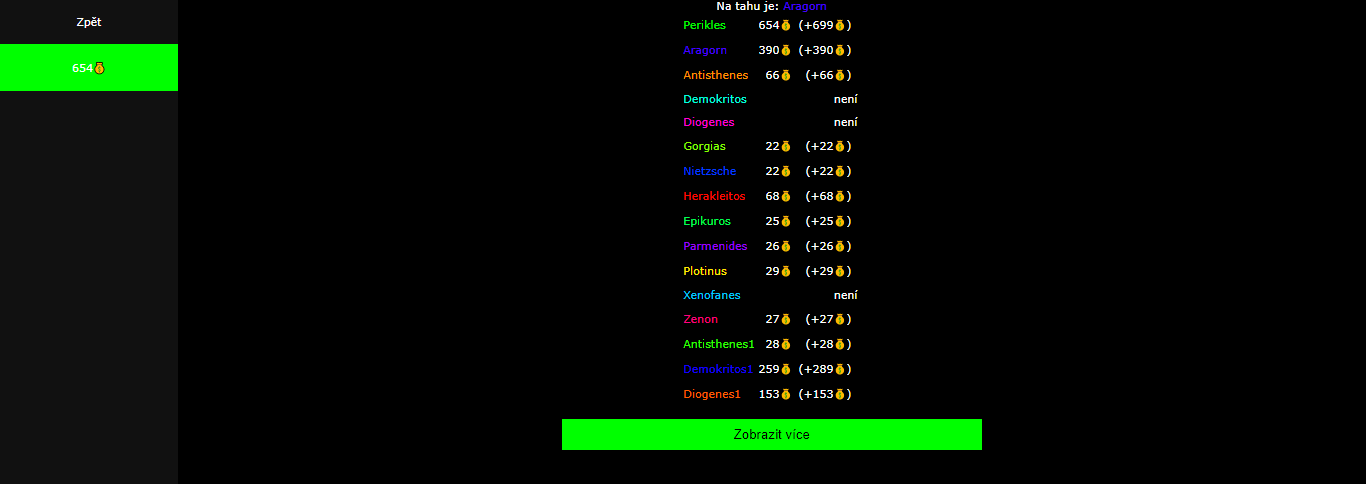
\includegraphics[width=\textwidth]{Players.png}

Po proběhnutí prvních několika tahů se pod možností vzdát se zobrazí tři grafy. První z~nich popisuje vývoj celkových sil hráčů (počítají se jako součet ceny všech vojáků, peněz, pětinásobku příjmů a stonásobku počtu cílových zemí, které daný hráč vlastní). Na druhém grafu se zobrazuje poměrná změna této síly. Na třetím se zobrazuje poměr vojenských sil hráčů (počítají se jako součet ceny všech vojáků a peněz) vůči sobě.

Na obrázku níže je ukázka prvního grafu ze hry, kterou vyhrál hráč, jenž má podle grafu až třetí největší sílu a jehož území zdaleka nebylo největší. Je tedy vidět, že při běžné hře k tomu může dojít.

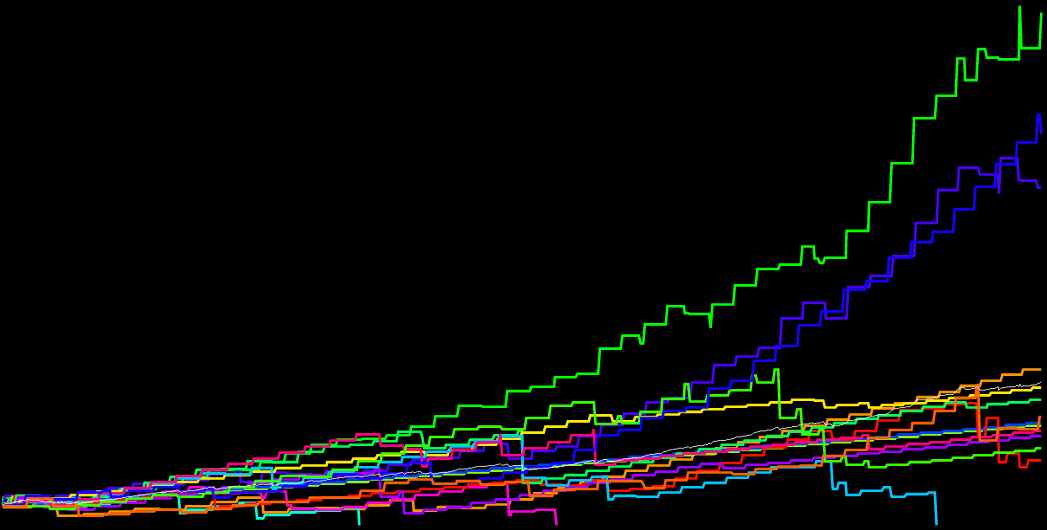
\includegraphics[width=\textwidth]{PowersGraph.png}

\section{Použité technologie}
\subsection{\CS{}}
Celý program je napsaný v~jazyce \CS{}, jelikož tento jazyk může běžet na straně serveru (viz ASP.NET Core) i klienta (viz Blazor WebAssembly) a obě části mohou využívat společné knihovny a pracovat s týmiž datovými typy. Navíc tento jazyk umožňuje využívat knihoven z~frameworku .NET a na rozdíl od jazyků PHP a JavaScript, které se často pro vývoj webových aplikací používají, je staticky typovaný a kompilovaný do bytekódu, což do určité míry kontroluje správnost programu.
\subsection{ASP.NET Core}
Framework ASP.NET Core je využíván na straně serveru ke zpracovávání HTTP dotazů a odesílání odpovědí.
\subsection{Blazor WebAssembly}
Blazor WebAssembly je framework, který umožňuje vyvíjet v~jazyce \CS{} aplikace spustitelné v~prohlížeči. Kód v~jazyce \CS{} se přeloží do binárního formátu WebAssembly a prohlížeč pomocí krátkého kódu v~JavaScriptu výsledný soubor stáhne a spustí. Spuštěný program následně reaguje na akce uživatele, komunikuje se serverem pomocí HTTP a podle potřeby překresluje zobrazovanou webovou stránku.

\section{Program}
Program se skládá ze tří projektů:
\begin{itemize}
\item\textit{Shared} -- Obsahuje třídy, které druhé dva projekty využívají, nachází se v~něm většina herní logiky a odpovídá větší části modelu v~architektuře MVC\cite{mvc}
\item\textit{Client} -- Odpovídá pohledu v~architektuře MVC a obsahuje soubory v~HTML, CSS a kód v~\CS{}, překládaný do WebAssembly a spouštěný v~prohlížeči klienta
\item\textit{Server} -- Implementuje webové API, jež odesílá odpovědi na dotazy klienta, a zahrnuje kód, který je potřebný k funkčnosti API, tedy práci s databází a s třídami z~projektu \textit{Shared}; v~architektuře MVC odpovídá kontroleru a části modelu
\end{itemize}

Graf závislostí mezi projekty:

\begin{tikzpicture}[node distance=2cm]
\node (shared) [block] {Shared};
\node (client) [block, right of=shared, xshift=2cm] {Client};
\node (server) [block, below of=shared] {Server};
\draw [arrow] (client) -- (shared);
\draw [arrow] (server) -- (shared);
\draw [arrow] (server) -- (client);
\end{tikzpicture}

\subsection{Shared}
Projekt \textit{Shared} obsahuje složku \textit{Conversion}, v~níž jsou třídy zajišťující načítání některých typů v~ostatních složkách z~formátu JSON nebo naopak zápis do tohoto formátu. Ve složkách \textit{Commands}, \textit{Config} a \textit{Data} jsou datové typy, které odpovídají různým jevům ve hře. Jedná se o neměnné datové typy a z~pohledu jazyka \CS{} jsou to záznamy (\textit{records}), nikoliv třídy. Dále je však budu označovat jako třídy, protože v~paradigmatu objektově orientovaného programování se skutečně o třídy jedná, neboť jejich instance obsahují data i funkce, které s těmito daty pracují.\cite{oop} Neměnné typy umožňují psát funkce a metody, které jsou referenčně transparentní (tj. nemají vedlejší účinky), a tím usnadňují přemýšlení o programu a snižují riziko chyb. \cite{immutable1}\cite{immutable2}

\subsubsection{Commands}
Ve složce \textit{Commands} se nachází rozhraní \textit{ICommand} a třídy, jež ho implementují. Každá z~nich odpovídá nějakému příkazu, který může hráč provést: nákup provincie, darování peněz, verbování vojáků, přesun vojáků, kapitulace a konec tahu. Rozhraní má dvě metody; obě přebírají jako paramtetry seznam hráčů a provincií, nastavení hry a hráče, jenž příkaz provedl. Jedna z~nich ověřuje, zda je příkaz možné provést a druhá jej provede a vrátí změněný seznam hráčů a provincií (aniž by měnila ten původní). Kód rozhraní vypadá takto:

\scriptsize\selectfont
\texttt{\keyword{public interface }ICommand}\\
\texttt{\{}\\
\hspace*{8mm}\texttt{\keyword{bool }Allowed(Player actor, IReadOnlyList<Player> players, Provinces provinces, Settings settings);}\\
\hspace*{8mm}\texttt{(IEnumerable<Player>, IEnumerable<Province>, Game) Perform(Player actor, IReadOnlyList<Player> players,}\\
\hspace*{48mm}\texttt{Provinces provinces, Settings settings, Game game);}\\
\texttt{\}}\normalsize

\subsubsection{Config}
Ve složce \textit{Config} se nachází třída \textit{Settings}, jež obsahuje data načtená při spuštění programu z~konfiguračního souboru a společná pro všechny hry. Instance ostatních tříd v~této složce jsou členské proměnné této třídy. Jsou zde třídy \textit{Land}, \textit{Sea} a \textit{Mountains}, odvozené z třídy \textit{Region} a uchovávající údaje o provinciích, jež se nemění v~průběhu hry: výnosy, výchozí armáda, popisek, tvar, barva, pravděpodobnost odtržení a zvláštní jednotky, verbovatelné v~provincii (například slon nebo fénická loď). Dále se ve~složce nachází třídy \textit{Pedestrian}, \textit{Elephant}, \textit{Ship} a \textit{OutlandishShip}, které dědí ze~třídy \textit{SoldierType} a reprezentují typy vojáků.

Graf hierarchie tříd pro data provincií:

\begin{tikzpicture}[node distance=2cm]
\node (region) [block] {Region};
\node (sea) [block, right of=region, xshift=2cm] {Sea};
\node (land) [block, below of=region] {Land};
\node (mountains) [block, below of=sea] {Mountains};
\draw [arrow] (sea) -- (region);
\draw [arrow] (land) -- (region);
\draw [arrow] (mountains) -- (region);
\end{tikzpicture}

Graf hierarchie tříd pro typy vojáků:

\begin{tikzpicture}[node distance=2cm]
\node (soldiertype) [block] {SoldierType};
\node (pedestrian) [block, below of=soldiertype] {Pedestrian};
\node (elephant) [block, below of=pedestrian] {Elephant};
\node (ship) [block, right of=pedestrian, xshift=2cm] {Ship};
\node (outlandishship) [block, below of=ship] {OutlandishShip};
\draw [arrow] (pedestrian) -- (soldiertype);
\draw [arrow] (ship) -- (soldiertype);
\draw [arrow] (elephant) -- (pedestrian);
\draw [arrow] (outlandishship) -- (ship);
\end{tikzpicture}

\subsubsection{Data}
Ve složce \textit{Data} se nacházejí třídy pro data, jež reprezentují stav hry, a proto se v průběhu stále mění. Přesto se však jedná o neměnné datové typy a změna se provádí nahrazením jednoho objektu za jiný. Dvě nejdůležitější třídy jsou \textit{Player} a \textit{Province}, které reprezentují o hráče a provincii. Kromě třídy \textit{Player} je zde také třída \textit{PlayerIdentity}, jež obsahuje hráčovo jméno, pořadí na tahu, hru a údaj, zda se jedná o lidského hráče či algoritmus, tedy informace, které hráče jednoznačně identifikují a nemění se během hry. Třída \textit{Player} následně obsahuje instanci třídy \textit{PlayerIdentity}, instanci třídy \textit{Settings}, protože metody třídy potřebují znát nastavení, počet peněz, heslo, údaje, zda hráč žije a zda je na tahu, a neměnný seznam prvků \textit{IAction}, jež obsahuje hráčem prováděné akce, jež se uskuteční při ukončení tahu. Kód rozhraní \textit{IAction}:

\scriptsize\selectfont
\texttt{\keyword{public interface }IAction}\\
\texttt{\{}\\
\hspace*{8mm}\texttt{(Player, Provinces, IAction?) Perform(Player active, Provinces provinces, Settings settings);}\\
\texttt{\}}\normalsize

Akce tedy podobně jako příkaz přebírá informace o stavu a vrací změněný stav. Třetí vrácená hodnota je potom akce, která v příštím kole nahradí v poli akcí hráče tuto akci, nebo hodnota \textit{null}, pokud má být tato akce bez náhrady odstraněna. Rozhraní \textit{IAction} implementují třídy \textit{Loan} a \textit{Manoeuvre}, které reprezentují splácení půjčky a přesun vojska. Třetí vrácená hodnota je u přesunu vojska vždy \textit{null}, neboť vojsko se vždy na konci tahu přesune, zatímco u půjčky se vrací opět půjčka, jejíž dlužná částka je zvýšená o úrok a snížená o splacenou částku, nebo \textit{null}, pokud již došlo ke splacení půjčky.

Třída \textit{Province} obsahuje instanci třídy \textit{Region}, jež uchovává základní a neměnné informace o provincii, a třídy \textit{Settings}, která je využívána v metodách. Dále obsahuje \textit{PlayerIdentity} hráče, jemuž provincie náleží, nebo hodnotu \textit{null}, pokud provincie žádnému hráči nepatří. Důvod, proč třída \textit{Province} obsahuje pouze identitu hráče a nikoliv přímo instanci třídy \textit{Player}, je ten, že ostatní údaje o hráči se mohou měnit, což by při použití neměnných datových typů vyžadovalo pokaždé přímo měnit všechny provincie změněného hráče, což by do kódu vneslo zbytečnou složitost, vzhledem k tomu, že ve třídě \textit{Province} je identita hráče použita pouze pro porovnání, zda hráč, který do provincie poslal vojenské jednotky je vládcem provincie, nebo se snaží provincii dobýt. Třída \textit{Province} ještě obsahuje objekt třídy \textit{Soldiers}, který reprezentuje současnou armádu v provincii a obsahuje neměnné pole typu \textit{Regiment}, což je třída obsahující instanci \textit{SoldierType} a počet vojenských jednotek onoho typu. Provincie jsou následně zapouzdřené ve třídě \textit{Provinces}, která obsahuje pole provincií a objekt třídy \textit{Graph}, v němž je uloženo, mezi kterými provinciemi vede cesta.

Mezi další třídy v této složce patří \textit{Game}, obsahující informace o stavu samotné hry, což je údaj o tom, zda hra již začala nebo skončila (a kdy se tak stalo), zda je nově vytvořená, nebo zda brzy začne (a kdy se tak stane). Síla hráče v daném kole se ukládá do třídy \textit{Power} a skládá se z počtu jeho čílových zemí, peněz, výše příjmů, síly vojáků a údaje, zda je hráč vůbec naživu. Hodnoty síly každého hráče pro dané kolo se ukládají do pole typu \textit{Power} ve třídě \textit{Powers}. Dále se ve složce nachází pomocné typy \textit{Ratio}, jež reprezentuje zlomek od $0$ do $1$, a \textit{Password}, jež reprezentuje hashované heslo. Třída \textit{Brain} obsahuje algoritmus hráče robota.

\subsection{Server}
V projektu \textit{Server} se nachází složky \textit{Controllers}, \textit{Files}, \textit{Pages}, \textit{Properties} a \textit{Services}. Složky \textit{Properties} a \textit{Pages} slouží pro potřeby frameworku ASP.NET Core. Ve složce \textit{Files} se nachází nastavení hry, načtená při spuštění do objektu \textit{Settings}, a SQL kód pro vytvoření tabulek v databázi. Ve složce \textit{Controllers} jsou třídy kontrolerů, jež jako parametry v konstruktoru dostanou objekty služeb, pomocí nichž získávají a zpracovávají data z databáze. Toho využívají k odpovídání na HTTP dotazy z klienta.

Složka \textit{Services} obsahuje třídy služeb, které zajišťují práci s databází a se třídami z projektu \textit{Shared}. Služby vždy implementují nějaké rozhraní a do metody ostatních tříd mají přístup jen k tomu rozhraní, aby se případná implementace mohla změnit. Připojení k databázi a provádění příkazů zaručuje rozhraní \textit{IDatabase}, které je v současnosti implementováno třídou \textit{SqliteDatabase} pro databáze Sqlite. Kdyby měla být v budoucnu nahrazena Sqlite databáze například databází MySQL, rozhraní by mohlo zůstat stejné a třídy, které databázi používají skrze něj, by zůstaly nedotčeny.

\subsection{Client}
V projektu \textit{Client} se nachází složka \textit{Pages}, v níž se nachází soubory Blazor komponentů. Každý takový soubor obsahuje kód v HTML i v \CS{} a reprezentuje určitou část stránky i její chování. Kód v \CS{} může být spouštěn při načtení stránky nebo při interakci s uživatelem a provádí změny stránky tím, že může části HTML zobrazovat jen při splnění určité podmínky, vytvářet HTML kód v cyklu nebo vyjádřit část HTML kódu jako hodnotu výrazu v \CS{} a při změně této hodnoty ji měnit. Navíc lze komponent použít jako HTML tag v jiném komponentu a tak rozdělit stránku do více souborů.

Ve složce \textit{Services} se nachází služby, které může kód v \CS{} využívat k posílání HTTP dotazů na server a přístupu k úložišti v prohlížeči a složka \textit{Data} obsahuje datové typy, které definují strukturu formátu JSON používaného při komunikaci se serverem a zápisu do úložiště. Složka \textit{Properties} obsahuje pouze konfigurační soubor \textit{launchSettings.json} pro potřeby frameworku Blazor. Ve složce \textit{wwwroot} se nachází soubory \textit{favicon.ico} a \textit{site.css}, které obsahují ikonu stránky a její CSS styly, a \textit{index.html}, což je krátký HTML soubor, který se zobrazí při načítání stránky a pomocí JavaScriptu načte a spustí aplikaci.

\section{Roboti}
Pokud se do hry zaregistruje méně než 16 hráčů, jsou hráči doplněni roboty. Robot je automaticky generovaný hráč, který hraje podle naprogramovaných pravidel.

\newpage
\printbibliography[heading=bibintoc, title={Použitá literatura}]
\end{document}